\section{Methods and Materials}
\label{sec:methods} 
en esta sección se describe la arquitectura del agente, el diseño de la función de recompensa y el protocolo de entrenamiento.
\begin{figure}[h]
    \centering
    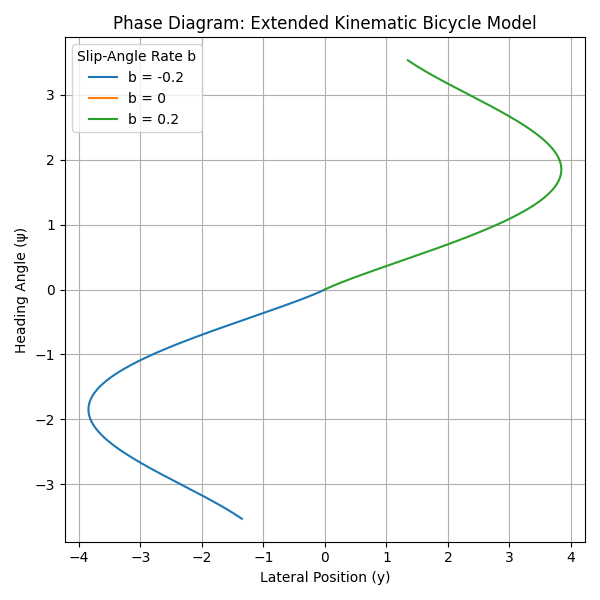
\includegraphics[width=0.8\linewidth]{images/bicylce_model1.png}
    \caption{Arquitectura del agente DRL.}
    \label{fig:arch} 
\end{figure}
La figura~\ref{fig:arch} ilustra la arquitectura del agente, que incluye un codificador multimodal, un decodificador y un módulo de control. El codificador multimodal fusiona datos LiDAR y características inerciales, mientras que el decodificador genera acciones continuas para el control del vehículo. El módulo de control implementa un algoritmo de aprendizaje por refuerzo profundo (DRL) para optimizar el rendimiento del agente en el entorno simulado.
\subsection{Arquitectura del agente}
Hola mi gente fffff
